\bookmark[dest=\HyperLocalCurrentHref,level=1]{Deep Learning Methods}
\section{Deep Learning Methods} \label{sec4}
Conventional physics-based reconstruction algorithms have been discussed above. In recent years, with the successful application of data-driven algorithms (e.g., deep learning\cite{lecunDeepLearning2015}) in blind deconvolution \cite{kupynDeblurGANBlindMotion2018}, depth estimation\cite{eigen_depth_2014}, and LOS imaging\cite{lindellSinglephoton3DImaging2018,su_deep_2018,marco_deeptof_2017}, recent works have also explored the possibility of deep learning in NLOS imaging. This section first explains the significance of using deep learning algorithms from a priori perspective, then introduces the end-to-end learning algorithms, as well as the hybrid algorithms that combine deep learning with physical models. Finally, we discuss the challenges and prospects of deep learning algorithms. 
Table~\ref{tab:deeplearning} summarizes the existing deep learning-based NLOS imaging technologies and their network, input, output, and training datasets.

\bookmark[dest=\HyperLocalCurrentHref,level=2]{Priors in NLOS imaging}
\subsection{Priors in NLOS imaging}
\label{sec:PriorsinNLOS}
Some priors have been effectively used in NLOS imaging, as reviewed below.


\vspace{0.8em}
\noindent\textbf{Non-negative prior.}
The non-negative prior includes two parts. First, for the optical transport matrix $\mathbf{A}$, by definition, the value of each element is non-negative; Second, for the reconstruction model based on the albedo $\rho$, the albedo of each voxel is also non-negative. The non-negativity of the light transport matrix and albedo $\rho$ together constitute non-negative prior.

\vspace{0.8em}
\noindent\textbf{Sparsity prior.}
Since the measurement data only contains the surface information of the hidden scene, which is sparse in the entire 3D space, the albedo (target scene) $\rho$ has a sparsity prior. A common sparse constraint is to directly use the $L_1$-norm constrain, i.e., $\|\rho\|_{1}$, and \cite{heideDiffuseMirrors3D2014} added different weights to each voxel. Another sparse constraint is a gradient constraint, which limits the gradient in the depth axis is sparse. The last type of sparsity constraint is that there should be only one non-zero value on the z-axis corresponding to each $(x, y)$ coordinate\cite{heideDiffuseMirrors3D2014}. Most NLOS reconstruction algorithms used sparse constraints as the main component of the regularization term $\Gamma(\rho)$\cite{heideNonlineofsightImagingPartial2017,Young:2020:dlct}.

\vspace{0.8em}
\noindent\textbf{Total variational (TV) prior.}
TV represents the sum of discrete gradients, and the TV regularization term is widely used in edge-preserving denoising\cite{rudin_nonlinear_1992,chambolle_introduction_2010} and sparse reconstruction of low-sample data(e.g., compressed sensing)\cite{tang_performance_2009}. For 3D NLOS reconstruction, TV prior represents the sparsity of hidden objects, especially sparsity on the z-axis, which is the gradient constraint discussed above. For two-dimensional NLOS imaging, the TV prior is mainly to restore the image from the inverse problem and maintain the edge information. Due to the effectiveness of the total variation constraint, many NLOS imaging studies have used the TV prior as the regularization term\cite{saundersComputationalPeriscopyOrdinary2019,wuNonLineofsightImaging2021,metzlerDeepinverseCorrelographyRealtime2020,tanakaPolarizedNonLineofSightImaging2020}.


\vspace{0.8em}
\noindent\textbf{Other priors.}
The above three types of priors apply to most NLOS imaging problems. Besides, there are some priors suitable for specific NLOS imaging. Specifically, for ToF-based NLOS imaging, the ellipsoid constraint\cite{otooleConfocalNonlineofsightImaging2018,veltenRecoveringThreedimensionalShape2012}, as well as the surface parameter constraint (e.g., the discontinuity of the ToF measurement contains the information of the surface normal)\cite{xinTheoryFermatPaths2019,tsaiGeometryFirstreturningPhotons2017} are two important priors. For NLOS imaging with partial occluders, the prior knowledge of the occluder's position and shape are also significant for high-quality reconstruction\cite{yedidiaUsingUnknownOccluders2019, thrampoulidisExploitingOcclusionNonLineofSight2018}. Besides, the BRDF prior also plays an important role in improving imaging results\cite{kadambiOccludedImagingTimeofflight2016}.

\bookmark[dest=\HyperLocalCurrentHref,level=3]{Unexploited prior -- scene prior}
\subsubsection{Unexploited prior -- scene prior}
However, there are still some priors that have not been effectively used. Therefore, using this undeveloped prior information is a meaningful way to improve NLOS imaging quality.

Scene priors is an important kind of unexploited priors, which includes both low-level features (e.g., smoothness) and high-level features (e.g., semantic information) of hidden scenes. Scene priors are particularly important for specific reconstruction tasks, such as NLOS imaging in autonomous vehicles or medical imaging.
Compared with other priors, most scene priors are implicit and difficult to extract manually. Therefore, conventional physics-based methods are challenging to formulate and efficiently utilize these scene priors.


The data-driven methods based on deep learning can learn the input data distribution, thereby efficiently completing the mapping from the input space to the output space, which has been utilized in a wide range of applications in recent years. For NLOS imaging, if there is enough reliable data, the data-driven methods can learn the scene prior effectively and improve reconstruction quality. Moreover, although the data-driven methods take a long time in the training phase and require high-performance computing hardware, it can almost achieve real-time processing in the test phase, which helps improve the real-time performance of NLOS imaging.

Limited by datasets and generalization, data-driven NLOS imaging research is still in the early stage. In recent years, several studies utilized deep learning to propose innovative reconstruction algorithms. The existing works can be roughly divided into two categories. One is to exploit the powerful representation ability of deep learning to build an end-to-end neural network directly (Fig.~\ref{fig:deeplearning}-(a)). The other is to combine the advantages of deep learning with physical models' constraints to improve imaging performance (Fig.~\ref{fig:deeplearning}-(b)).

\begin{figure*}[!h]
    \centering
    \includegraphics[width=1\textwidth]{./pic/Fig6_DeepLearning.pdf}%
    \caption{Two types of models of NLOS imaging based on deep learning: (a) End-to-End Networks. (b) Physics-based Models. The reconstruction results in \cite{chen_learned_2020} and \cite{zhouNonlineofsightImagingPhong2020} are used as a demonstration.}
    \label{fig:deeplearning}
\end{figure*}


\bookmark[dest=\HyperLocalCurrentHref,level=2]{End-to-End algorithms}
\subsection{End-to-End algorithms} \label{endToEnd}
NLOS imaging can be expressed as an inverse problem, as shown in Eq.~(\ref{inverse}). Therefore, an end-to-end deep learning model can be built, where the input is the measurement (e.g., $\tau$), and the output is the reconstruction of the hidden scene (e.g., $\hat{\rho}$). Then, a loss function is used to measure the difference between the output $\hat{\rho}$ and ground truth $\rho$, followed by back-propagation used to optimize the network weights, and finally, a good reconstruction result can be obtained. 

Most of the existed NLOS imaging works based on deep learning used the end-to-end network structure, as reviewed in Tab.~\ref{tab:deeplearning}. Chen \etal~used conventional cameras and continuous laser illumination to collect steady-state NLOS imaging data and corresponding hidden scenes~\cite{chenSteadystateNonLineofSightImaging2019}. After that, a U-Net~\cite{ronnebergerUnetConvolutionalNetworks2015a}~based network was trained to complete the mapping from the measurement to the corresponding hidden scenes. In \cite{chenSteadystateNonLineofSightImaging2019}, the loss function was a multi-scale (for different resolutions) $L_2$ loss function.
Similarly, \cite{zhouNonlineofsightImagingPhong2020} and \cite{yuNonLineofSightImagingDeep2019} used the U-Net based network structure, with cross-entropy and ordinary $L_2$ norm as loss function to complete the passive NLOS imaging in Fig.~\ref{fig:introFig}-(c) and (d). They achieved better imaging performance than conventional methods\cite{tanakaPolarizedNonLineofSightImaging2020,saundersComputationalPeriscopyOrdinary2019}, as shown in Fig.~\ref{fig:passive}-(b).
For ToF-based transient NLOS imaging scenes, Chopite \etal~synthesized a large number of training images through rendering and noise models, and modified part of the input and output in U-Net from 2D tensor to 3D tensor using $L_2$ loss\cite{chopiteDeepNonLineofSightReconstruction2020}. Finally, based on the end-to-end deep neural network, \cite{chopiteDeepNonLineofSightReconstruction2020} completed the mapping from transient measurement to depth map.

\vspace{0.8mm}
\noindent \textbf{Direct NLOS photography.}
Most active transient methods optimize an intermediate hidden volume, depth map, or surface before producing a human-interpretable image. Peng~\etal~instead formulated NLOS photography as direct synthesis of a two-dimensional view from the relay-wall viewpoint~\cite{pengTowardsNLOSPhotography2021}. Their data-driven model maps measured transient transport directly to a high-resolution photograph, bypassing explicit three-dimensional geometry and allowing a relatively small training set. This change of target complements LCT, $f$--$k$, phasor-field, and neural-field reconstruction: it treats hidden texture and appearance as first-class outputs rather than secondary attributes of a recovered volume, anticipating later learned systems that optimize perceptual fidelity in addition to geometric accuracy.

In addition to reconstruction tasks, recognition is also an important goal in NLOS scenes. Due to the limited capability of conventional algorithms in high-level semantics, NLOS recognition mainly uses data-driven end-to-end algorithms based on deep learning. Lei \etal~completed the recognition of MNIST~\cite{lecunGradientbasedLearningApplied1998a} and human posture under different NLOS settings~\cite{leiDirectObjectRecognition2019}. \cite{caramazzaNeuralNetworkIdentification2017} showed that the deep neural network can classify and recognize hidden scenes with only one SPAD scanning point. In addition, a recent study~\cite{isogawaOpticalNonLineofSightPhysicsBased2020} has combined LSTM~\cite{hochreiterLongShortTermMemory1997} and physical models to complete 3D human pose estimation. Besides, Satat \etal~used deep neural networks to complete object classification through scattering media\cite{satatObjectClassificationScattering2017}.
For passive NLOS scenes, Tancik \etal~utilized CNN for positioning and recognition, achieving a high recognition accuracy\cite{DBLP:journals/corr/abs-1810-11710}. Besides, \cite{DBLP:journals/corr/abs-1810-11710} also explored the use of variational autoencoder (VAE)\cite{kingma_auto-encoding_2014} to complete NLOS reconstruction.
Du~\etal~designed a parallel encoder architecture for passive NLOS reconstruction that simultaneously processes multi-scale spatial features of the passive scattering measurement, enabling improved reconstruction fidelity with lower computational overhead compared to single-path encoder designs~\cite{du2025passive}. For joint NLOS scene understanding, Wang~\etal~proposed NLOS-R~2, which alternates between reconstruction and recognition in a mutual-refinement loop: semantic predictions from the recognition branch feed back as structural priors to sharpen reconstruction, while the improved reconstruction in turn enhances recognition accuracy~\cite{wang2025nlos}. This alternate training strategy achieves superior performance on both reconstruction and recognition tasks simultaneously, demonstrated on IEEE ICME 2025.


\bookmark[dest=\HyperLocalCurrentHref,level=2]{Network combined with physical models}
\subsection{Network combined with physical models} \label{combined}
The end-to-end method is convenient for training, but it is highly dependent on the dataset. When the dataset scale is large enough, end-to-end learning can learn the mapping well to achieve good results. However, end-to-end learning may have problems such as over-fitting and poor generalization ability when the data size is insufficient. Due to the cumbersome data acquisition process, NLOS imaging lacks real large-scale datasets (most of the existing large-scale datasets are synthetic). Hence, some state-of-the-art studies in recent years proposed a reconstruction algorithm combining deep learning and physical models instead of the end-to-end network only, as shown in Tab.~\ref{tab:deeplearning}.

Metzler \etal~used the optical memory effect (see Sec.~\ref{sec3}-\ref{memoryEffect1}) to complete NLOS imaging~\cite{metzlerDeepinverseCorrelographyRealtime2020}. Instead of using conventional phase recovery algorithms (e.g., hybrid input-output (HIO)~\cite{fienupPhaseRetrievalAlgorithms1982} and alternating minimization (Alt-Min)\cite{netrapalli_phase_2015}), \cite{metzlerDeepinverseCorrelographyRealtime2020}~adopted U-Net to complete phase recovery, with the $L_1$ norm after autocorrelation as loss function.
\vspace{0.8mm}
\noindent \textbf{Shared learned representations for reconstruction and recognition.}
Chen~\etal~introduced a learned feature-embedding framework that maps transient measurements into a common hidden-scene representation and then specializes it for high-resolution image reconstruction, classification, and 2.5D object detection~\cite{chen_learned_2020}. Rather than relying on a monolithic U-Net, the architecture incorporates differentiable modules with explicit physical roles, including transient propagation, visibility reasoning, image rendering, and depth estimation. Training on synthetically rendered diffuse and specular scenes while evaluating on measured transients demonstrated useful synthetic-to-real generalization. This work marks an early shift from single-output NLOS inversion toward reusable, task-aware representations, anticipating later physics-guided multi-task networks, transient pretraining, and transformer/operator models.

\vspace{0.8mm}
\noindent \textbf{Learnable inverse kernels and attention.}
Yu~\etal~subsequently made the inverse operator itself trainable by introducing a learnable inverse kernel tailored to the transient NLOS point-spread function, together with attention mechanisms for recovering hidden intensity and depth~\cite{yuLearnableInverseKernel2023}. The method remains explicitly tied to the active transient forward model while allowing data-driven adaptation beyond a fixed analytic inverse. In the learned-reconstruction trajectory, it provides an intermediate step between the shared, task-aware feature embeddings of Chen~\etal~and later spatial--temporal transformers or adaptive physical-prior networks: physics determines the operator structure, whereas learned kernels and attention determine how measurement evidence is inverted and emphasized.
\vspace{0.8mm}
\noindent \textbf{Learning the light-cone inverse.}
The original LCT obtains computational efficiency from a closed-form resampling and Wiener-deconvolution pipeline, but fixed low-pass filtering can suppress fine geometry. Gao~\etal~proposed a learned light-cone transform (L2CT) that retains the analytic LCT structure while replacing its frequency response with high-frequency-enhanced learnable Wiener filtering and adding spatiotemporal feature-extraction and volume-projection modules~\cite{gaoLearnedLCT2026}. Its improvement on measurements from different acquisition systems illustrates a useful middle ground between fixed analytic inverses and unconstrained end-to-end networks: the milestone operator remains recognizable, while the poorly conditioned spectral components are learned from data.

\vspace{0.8mm}
\noindent \textbf{Diffusion-based transient video interpolation.}
Dynamic NLOS systems face coupled spatial and temporal undersampling before reconstruction begins. Sun~\etal~introduced TransVID, which uses a spatial--temporal attention encoder and latent conditional diffusion to interpolate transient videos jointly across scan position and time~\cite{sunTransVID2026}. The method maps $16\times16$ measurements at 4~fps to $128\times128$ transient videos at 16~fps, providing a measurement-domain complement to ST-Mamba and TransiT: instead of reconstructing hidden video directly from sparse captures, it first synthesizes a dense, high-frame-rate transient sequence that can feed existing physical or learned inverses.

\vspace{0.8mm}
\noindent \textbf{SPAD-aware physics-informed cascade learning.}
Zhao~\etal~addressed the coupling between detector noise and ill-posed transient inversion with physics-informed cascade learning (PICL)~\cite{zhaoPICL2026}. A lightweight first network separates SPAD-specific dark-count, timing-jitter, and mixed interference components, after which a second network reconstructs the hidden scene while embedding a differentiable forward model. Because physical measurement consistency supplies self-supervision, PICL avoids dependence on a large paired NLOS dataset and provides a direct bridge from trainable inverse kernels toward hardware-aware, noise-adaptive reconstruction.

Another example of exploiting deep learning to promote the development of NLOS imaging is LiDAR-based imaging~\cite{zhuFastNonlineofsightImaging2021a}.
For traditional physical models, using commercial LiDAR as the equipment is still a very challenging problem. However, the recent work of Zhu \etal~showed that by performing deep learning to complete feature extraction, LiDAR can be used to complete high-quality and robust 3D NLOS reconstruction\cite{zhuFastNonlineofsightImaging2021a}.

Aittala \etal~regarded the measurement data as the product of the hidden object and the light transport matrix\cite{aittalaComputationalMirrorsBlind2019} (as shown in Eq.~(\ref{eq2_1})). Exploiting deep neural models to generate matrices satisfied matrix decomposition completes passive NLOS imaging based on unsupervised learning.
\cite{shenNonlineofsightImagingNeural2021} used unsupervised learning to complete active NLOS imaging. Specifically, \cite{shenNonlineofsightImagingNeural2021} exploited multilayer perceptron layers (MLP) to construct a neural transient field that maps measurement data into a hidden scene, and utilized a physical model to constrain the results, thereby obtaining superior reconstruction results.
Technically, such unsupervised learning methods~\cite{aittalaComputationalMirrorsBlind2019,shenNonlineofsightImagingNeural2021} are not data-driven methods, but the idea of using deep neural networks to simulate matrix factorization is instructive.

Recent works have significantly extended this paradigm of combining physical constraints with deep learning.


\vspace{0.8mm}
\noindent \textbf{Learning from under-scanned transients.}
Dense relay-wall scanning remained a practical acquisition bottleneck even after analytic reconstruction became fast. Li~\etal~introduced the first deep pipeline designed specifically for under-scanning measurements, coupling a transient recovery network that maps sparse scans to a dense measurement grid with a volume reconstruction network that embeds the linear light-path transport operator~\cite{liDeepNLOSUnderscanning2023}. Multi-kernel feature extraction and fusion recover measurement structure, while regularized constraints preserve local detail and suppress oversmoothing. The method remains effective for $8\times8$ confocal scans and reports approximately $50\times$ faster inference than an iterative under-scanning baseline. This work shifts learned active NLOS from post-reconstruction refinement toward joint measurement completion and physics-aware inversion, preceding later signal-superresolution, virtual-scanning, diffusion, and transient-transformer approaches.

\vspace{0.8mm}
\noindent \textbf{Neural implicit surfaces.}
Extending the neural transient field (NeTF)~\cite{shenNonlineofsightImagingNeural2021} to surface representations, Fujimura~\etal~proposed NLOS-NeuS~\cite{fujimuraNLOSNeuS2023}, which represents the hidden scene as a neural implicit surface via a signed distance function (SDF). By introducing SDF constraints based on first-returning photon geometry and volume rendering, NLOS-NeuS reconstructs smooth and detailed 3D surfaces without voxel resolution limitations, representing a major step towards high-fidelity 3D NLOS scene understanding.

\vspace{0.8mm}
\noindent \textbf{Learnable physical priors.}
Sun~\etal~introduced a framework with learnable physical priors~\cite{sunGeneralizable2025}, replacing manually designed fixed priors (such as single fixed path compensation) with adaptive priors learned from data. This enables significantly better generalization to diverse scene conditions and varying SNR levels, addressing the limited generalization capability that has been a persistent challenge for physics-based deep NLOS methods.

\vspace{0.8mm}
\noindent \textbf{Diffusion model priors.}
Su~\etal~proposed a model-guided iterative diffusion sampling approach for NLOS reconstruction~\cite{suModelGuidedDiffusion2024}, where the physical forward model of NLOS imaging guides the diffusion sampling process to generate reconstructions that satisfy measurement constraints while leveraging the strong generative prior of a pre-trained diffusion model. This approach achieves state-of-the-art NLOS reconstruction quality, demonstrating that diffusion models are a powerful new tool for solving the NLOS inverse problem.

\vspace{0.8mm}
\noindent \textbf{Plug-and-Play for dynamic NLOS.}
Ye~\etal~introduced a plug-and-play (PnP) framework for dynamic NLOS video reconstruction~\cite{yePnPDynamic2024}, incorporating a frequency-filtering step based on wave physics and a pre-trained deep neural network denoiser as an implicit prior. The flexible PnP structure allows easy integration of different denoisers and adapts to different NLOS imaging configurations, achieving superior temporal consistency over existing frame-by-frame reconstruction methods.

\vspace{0.8mm}
\noindent \textbf{Unsupervised reconstruction from irregular measurements.}
Cui~\etal~proposed Virtual Scanning~\cite{cuiVirtualScanning2024}, an unsupervised framework for NLOS imaging from irregularly undersampled transients (IUT) that does not require paired training data. A virtual scanning process enables the network to learn within both the range and null spaces of the measurement operator, combined with a physics-guided SURE-based denoiser for robustness to noise. This method achieves higher fidelity and orders-of-magnitude faster inference than existing iterative solutions.

\vspace{0.8mm}
\noindent \textbf{Aperture-limited diffusion and physics-guided high-speed reconstruction.}
TransDiff~\cite{cuiTransDiffTIP2025} extends unsupervised transient completion to aperture-limited relay surfaces using a latent diffusion prior constrained by the measured transients. In parallel, Physics to the Rescue~\cite{muPhysicsRescueTPAMI2025} embeds wave-propagation and volume-rendering priors into a neural reconstruction pipeline, improving robustness when high-speed acquisition requires approximate light-transport models. Together, these methods mark a shift from purely data-driven inversion toward learned solvers whose latent completion is explicitly checked against transient physics.

\vspace{0.8mm}
\noindent \textbf{Untrained network priors.}
Wu~\etal~demonstrated that an untrained deep decoder network can serve as an effective image prior for NLOS reconstruction without any training data~\cite{wuUntrainedDecoder2022}, leveraging the deep image prior inherent in the network architecture to regularize the ill-posed NLOS inverse problem, offering flexibility for novel experimental configurations where training data is unavailable.

\bookmark[dest=\HyperLocalCurrentHref,level=2]{Challenges and Prospects}
\subsection{Challenges and Prospects}
NLOS imaging based on deep learning still faces many challenges, including lack of datasets, lockstep network structure, and limited generalization capability. Here, we discuss these three challenges and the corresponding prospects separately.


\bookmark[dest=\HyperLocalCurrentHref,level=3]{Dataset}
\subsubsection{Dataset}
Data-driven algorithms' performance largely depends on the dataset's quality (such as scale and reliability). However, for transient NLOS imaging, acquiring a sample of data requires a raster scan of the imaging area, which takes about 1 to 5 minutes~\cite{otooleConfocalNonlineofsightImaging2018,isogawaEfficientNonLineofSightImaging}. Therefore, constantly changing hidden objects and collecting tens of thousands of measurements to form a large-scale dataset is extremely difficult. For NLOS imaging scenes based on traditional cameras, although data collection is less time-consuming, it is still complicated to continuously change scenes and construct large-scale dataset because data augmentation operations such as crop and flip are not suitable for NLOS imaging.

Most existing works construct a rendering model to synthesize datasets for training, i.e., they first use public datasets in other fields as the hidden object (ground truth) and then synthesize measurement data through a rendering model. For transient NLOS imaging, the rendering model includes two parts: transient rendering and sensor model~\cite{chen_learned_2020,chopiteDeepNonLineofSightReconstruction2020}. The SPAD-based photon calculation model has been studied in detail, and they take into account factors such as noise, crosstalk and afterpulsing~\cite{hernandez_computational_2017}. For other types of NLOS imaging, Metzler \etal~used Berkeley Segmentation Dataset 500~\cite{martin_database_2001} as a hidden scene to calculate autocorrelation, which is then used to train the phase recovery network~\cite{metzlerDeepinverseCorrelographyRealtime2020}. For passive NLOS imaging using traditional cameras and ambient light, diffuse surface illumination models, such as the Phong Model~\cite{phongIlluminationComputerGenerated1975}, can be used for rendering to obtain synthesized passive NLOS data~\cite{zhouNonlineofsightImagingPhong2020}. 

Due to the sensitivity of deep learning algorithms to abnormal data, improving the accuracy of rendering models is extremely important to data-driven NLOS imaging methods. Another alternative is designing an automated/real-time data collection system to collect data in the experimental setup.

Since 2022, dedicated NLOS rendering tools have emerged to generate higher-fidelity synthetic training data. Royo~\etal~presented the first NLOS transient renderer designed to accurately simulate light transport in NLOS scenarios, enabling generation of realistic training data and testing of reconstruction algorithms~\cite{royoNLOSTransientRendering2022}. Plack~\etal~subsequently developed a fast differentiable transient renderer for NLOS scenes that supports automatic differentiation, enabling gradient-based optimization of scene parameters and end-to-end training of NLOS reconstruction networks~\cite{plackFastDifferentiable2023}. For passive NLOS tracking, Wang~\etal~released the NLOS-Track dataset, the first large-scale dynamic passive NLOS tracking dataset with thousands of real and synthetic video clips paired with trajectory labels~\cite{wangPropagateCalibrate2023}, addressing the severe data scarcity problem in passive NLOS research.

Complementing physically complete transient renderers with a benchmark-oriented alternative, Shi~\etal~introduced a configurable simulator grounded in the light-cone transform and accelerated by three-dimensional FFT convolution~\cite{shiFastNLOSTransientSimulation2025}. The framework accepts depth and optional albedo maps, exposes relay-wall extent, stand-off distance, temporal binning, detector jitter, and Poisson noise as explicit parameters, and releases transient data for seven ShapeNet object categories together with common LCT, phasor-field, $f$--$k$, and backprojection baselines. This development lowers the cost of standardized algorithm comparison and large-scale learning, while remaining complementary to Monte Carlo transient rendering when higher-order transport, complex materials, or full sensor realism are required.

\begin{figure*}[!h]
    \centering
    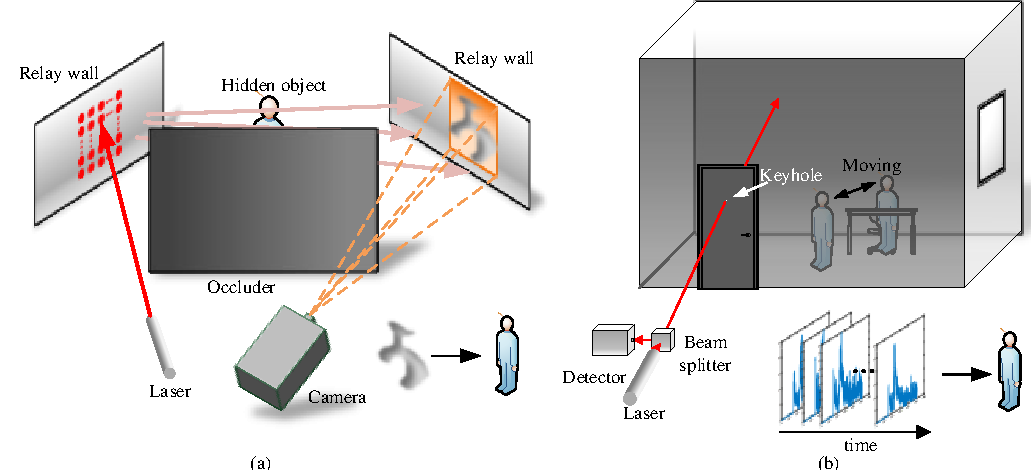
\includegraphics[]{./pic/Fig7_newnlos.pdf}%
    \caption{New NLOS scenes. (a) Two bounce NLOS imaging. (b) Keyhole NLOS imaging. }
    \label{fig:newNLOS}
\end{figure*}

\bookmark[dest=\HyperLocalCurrentHref,level=3]{Network Architecture}
\subsubsection{Network Architecture}
According to Sec. IV~\ref{endToEnd} and \ref{combined}, most NLOS imaging networks currently use the classic network structure (or with tiny changes), such as U-Net~\cite{ronnebergerUnetConvolutionalNetworks2015a} and ResNet~\cite{heDeepResidualLearning2016a}. However, these well-known network structures are not necessarily suitable for NLOS imaging. Compared with recent works in other inverse problems, such as low-light image recovery~\cite{liu_pd-gan_2021} and image deblurring~\cite{rozumnyi_defmo_2020}, networks designed for specific tasks achieve better results. Therefore, it can be expected that in the future, more novel network architectures based on the characteristics of NLOS imaging(e.g., \cite{chen_learned_2020}) will be proposed to improve the performance of NLOS imaging.

Since 2022, the NLOS community has indeed witnessed a wave of new architectures designed specifically for the challenges of 3D transient imaging.

\vspace{0.8mm}
\noindent \textbf{Transformer-based networks.}
Li~\etal~proposed NLOST~\cite{liNLOST2023}, the first transformer specifically designed for NLOS 3D reconstruction. NLOST uses spatial-temporal self-attention at multiple scales to capture both local and global correlations within the high-dimensional transient measurement volume, achieving superior performance on real-world confocal and non-confocal data. For NLOS videography, Li~\etal~developed TransiT~\cite{liTransiT2025}, a transient transformer architecture that directly compresses the temporal dimension of input transients to extract features efficiently at high frame rates, combining feature fusion and spatial-temporal attention with transfer learning to bridge the synthetic-to-real gap.

\vspace{0.8mm}
\noindent \textbf{State-space model (Mamba) for video NLOS.}
Li~\etal~proposed ST-Mamba~\cite{liMambaTemporalConsistency2024}, the first spatial-temporal Mamba model for dynamic NLOS reconstruction. ST-Mamba exploits the time-resolving causality in transient measurements through interleaved Mamba blocks, incorporating a wave-based loss function in the phasor field domain to handle measurement noise in NLOS video. This approach achieves superior temporal consistency across frames compared to per-frame reconstruction methods.

\vspace{0.8mm}
\noindent \textbf{Graph neural networks.}
Su~\etal~proposed DG-NLOS~\cite{suDGNLOS2025}, which employs a graph neural network (GNN) as its fundamental component to transform dense NLOS grid data into sparse structural features. DG-NLOS uses a dual-branch architecture with one branch dedicated to albedo recovery and another for depth/geometry, enabling simultaneous reconstruction of appearance and structure with reduced computational and memory cost. To the authors' knowledge, DG-NLOS is the first work to employ GNNs as a core module for NLOS reconstruction.

\bookmark[dest=\HyperLocalCurrentHref,level=3]{Generalization}
\subsubsection{Generalization}
Limited by the dataset and network structure discussed above, current data-driven NLOS imaging algorithms have limited generalization capabilities. \cite{chopiteDeepNonLineofSightReconstruction2020} and \cite{chen_learned_2020} can get good test results on the public NLOS data~\cite{galindoDatasetBenchmarkingTimeresolved2019,otooleConfocalNonlineofsightImaging2018} through training on the synthetic training set, which means that they have a certain generalization ability. However, this does not mean that the generalization capabilities of current algorithms are sufficient. Faced with new parameters (such as BRDF, time jitter, aperture size) and new hidden scenes that do not exist in the training dataset, the trained network may not necessarily achieve acceptable results.

The most two direct ways to increase the generalization ability are improving the dataset's quality and the network structure, as discussed above. Another method is to use transfer learning so that a network trained on one kind of data can be quickly transferred to another kind of data. Besides, unsupervised learning is also a promising method. It does not rely on large amounts of data, but can use deep neural networks' powerful representation capabilities to train a model that meets the physical constraints (e.g., the optical transport matrix in~\cite{aittalaComputationalMirrorsBlind2019}), which has more substantial generalization capabilities.

Recent advances have made meaningful progress on the generalization problem. Sun~\etal~proposed a framework with learnable physical priors~\cite{sunGeneralizable2025} that adapts to diverse imaging conditions automatically, demonstrating substantially improved generalization across different SNR levels and scene configurations. Domain reduction strategies~\cite{shimDomainReduction2024} that focus the reconstruction search space on the most likely hidden object locations also improve both speed and generalization. Transfer learning has been successfully applied in TransiT~\cite{liTransiT2025} to bridge the synthetic-to-real domain gap for NLOS videography. Looking forward, the combination of physics-constrained learning, untrained priors~\cite{wuUntrainedDecoder2022}, and self-supervised approaches~\cite{cuiVirtualScanning2024} holds promise for enabling robust NLOS reconstruction even without large-scale real training data.

\bookmark[dest=\HyperLocalCurrentHref,level=2]{Dynamic NLOS Imaging}
\subsection{Dynamic NLOS Imaging}
\label{sec:dynamicNLOS}
Real-time reconstruction of dynamic hidden scenes is one of the most practically significant challenges in NLOS imaging, and it has seen remarkable progress since 2022. The main bottleneck is that dense raster scanning limits the practical frame rate to well below real-time, creating a fundamental tension between acquisition density and temporal resolution.

Towards resolving this tension, several strategies have emerged. Ye~\etal~demonstrated real-time NLOS video at 4\,fps for room-sized scenes by combining spectrum filtering (denoising/deblurring in the frequency domain) with an interleaved scanning scheme that computes high-resolution live video from low-quality sequences acquired during scanning~\cite{yeRealTimeNLOS2024}. Li~\etal~proposed ST-Mamba~\cite{liMambaTemporalConsistency2024}, which exploits temporal consistency across frames using spatial-temporal Mamba blocks and a wave-based phasor field loss to reconstruct high-resolution NLOS volumes from under-scanning transient videos. For videography with a transient transformer, TransiT~\cite{liTransiT2025} achieves 10\,fps reconstruction at $64\times64$ resolution from $16\times16$ sparse transients captured at 0.4\,ms exposure per point, demonstrating practical video NLOS reconstruction on real hardware. Ye~\etal~further developed a plug-and-play algorithm for dynamic NLOS video~\cite{yePnPDynamic2024} that combines frequency-domain physics filtering with a deep denoiser prior, enabling flexible and high-quality reconstruction of moving hidden scenes.
